\chapter{Experimental Evaluation}

\noindent For the purposes of evaluating Modulo7, test cases have been designed into two formats. One category of testing is micro testing, for validating correctness and precision recall for small sets of data. This ensures verifiability of algorithms and similarity measures on small datasets as well as novel explorations of data. Most MIR research is done on small scale datasets and hence falls in the purview of micro testing. The other format is macro testing which involves larger datasets such as the million song dataset \cite{msd}. Due to computing resource c, subsets of larger datasets were chosen such that memory and disk requirements could be  contained in one PC. No distributed test cases were run as a part of the evaluations. \\\\
A few assumptions that are made in testing are as follows :-
\begin{enumerate}
\item In order to estimate ground truth values, ground truth values presented in datasets (such as tagged meta data or subjective jugdments for song similarity ) are assumed as a base line.
\item If the song meta data (such as key-signature, time-signature, total duration of song) is not encoded, its estimated by the individual parsers for the data source. This estimation is done by existing algorithms in literature. However if meta data is encoded in the input, its assumed to be correct and no such estimations are carried out. 
\item Most tests are against file formats of similar types (for example midi is tested against other symbolic files). This is due to the inherent complexity of symbolic decoding of audio formats like mp3.
\item In the event of parsing data, there can be legal issues (e.g. the song can be copyrighted). For that reason custom parsers are built for alternate research dataset format (e.g the million song dataset has already derived features that Modulo7 intended to derive for Mp3 files and has its own parser written by the creators of the data sets. \cite{msd})
\item All evaluations are done against research datasets which are published in academia or exposed as public data sets in industry. As such no proprietary data sets are used for the purpose of any evaluation metric.
\end{enumerate}

\section{Results of Index Compression}

\noindent The Modulo7 representation can be thought of an indexed meta data version of the song with the symbolic information of the song intact(which entails no core information is lost during the conversion). True to all indexed data, Modulo7 represents the song in a much smaller size than the original source. The following chart demonstrates the average compression of indexed data as compared to source files on the Saarland Music Data (SMD) Dataset \cite{saarlandmsd} when the modulo7 representation is persisted on disk:-
\begin{figure}
\centering
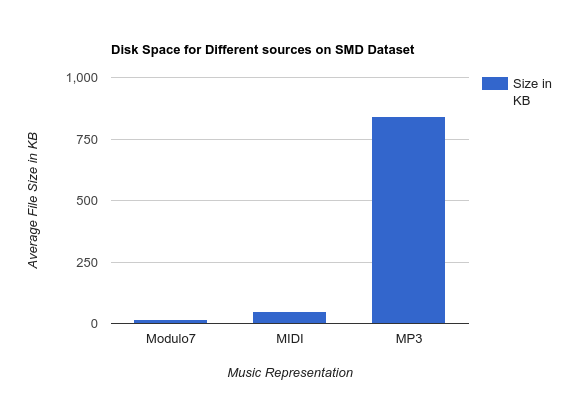
\includegraphics[width=\textwidth]{Modulo7SMDBarGraph.png}
\makeatletter
\let\@currsize\normalsize
\caption{Modulo7 architectural design}
\label{fig:figure}
\end{figure}
As expected Modulo7's serialized format expresses a song in less disk space than its source formats while keeping the symbolic information intact. The results are positive as there is a 4 time decrease in size of expressing symbolic information as compared to midi files. \\\\
A similar transformation was also done on a direct download able subset of the wikifonia dataset in order to compare Modulo7 internal representation against the compressed xml representation of the wikifonia dataset. A plot of disk space requirements are plotted in ascending order of the wikifonia dataset file sizes:- 
\begin{figure}
\centering
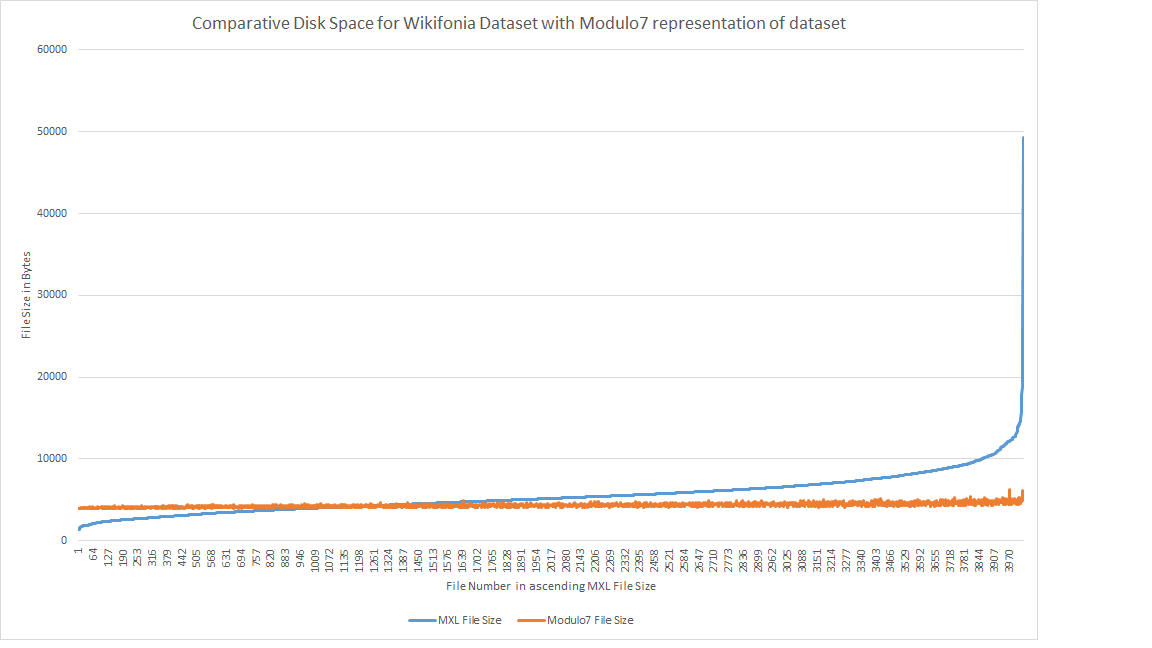
\includegraphics[width=\textwidth]{M7Graph.png}
\makeatletter
\let\@currsize\normalsize
\caption{Modulo7 comparative file sizes}
\label{fig:filesizes}
\end{figure}

\noindent As expected, Modulo7 is extremely space efficient for storing symbolic information.
\section{Million Song Dataset Experiments}

\noindent The million song dataset was chosen for experimental evaluation \cite{msd}. MSD contains pre-computed symbolic transcriptions of Mp3 files and the last fm data set for ascertaining similar songs to build a ground truth for evaluation. Due to the constraints of hardware for evaluation, we took a scaled down subset of the original 584,897 songs to a more manageable 10000 songs(offered as a direct down loadable subset in the Million song data set website \cite{msddownloadable}), with similar songs edited to fit this dataset. This data set is used for both melodic similarity computation and exploratory querying for determining best fit queries for certain criteria.

\subsection{Results on melodic similarity analysis}

\noindent This set of experiments determine the precision and recall values for the similarities defined in \ref{similarity} on ground truth data extracted from \cite{msd}. Modulo7 does not claim to improve on the state of the art when it comes to similarity metrics or does not intend to create a new similarity metric. Rather this set of experiments are a test of efficiency in execution and accuracy of existing methods on large scale datasets. \\

\noindent For this experiment the songs that they were monophonic are retained(since polyphonic transcription from audio files is not a fully solved problem \cite{melextract}) and a subset of 3,784 songs are retained. These songs were mapped with the last fm similarity dataset and 838 songs out of the monophonic subset were identified to have at least one similar song listed in the last fm tags. This final subset was treated as the ground truth for this experiment. \\

\noindent Only the monophonic similarity measures are used for these experiments from \ref{monophonicSim}. The testing was done with a 10\% test set (search queries) and 90\% hold out set (data base) and 10 fold cross validation was used. \\

\noindent In order to estimate a song similarity ground truth that faithfully captures the user's sentiment about a song, a quantitative estimate was designed around the meta data associated with a song called the tag hit rate. Given a song $S_1$ with tags $T(S_1)$ and another song $S_2$ with tags $T_(S_2)$. The tag hit rate is defined as :-

\begin{equation} \label{taghitrate}
THR(S_1, S_2) = \sum_{t_i \in T(S_1)} \sum_{t_j \in T(S_2)} \begin{cases} 
      1 & t_i == t_j \\
      0 & otherwise \\  \end{cases}
\end{equation}

\noindent This can be interpreted as an quantitative estimate of the agreement between tags of two songs, and as a consequence the song similarity based on a collaborative filtering approach. \\

\noindent Based on this measure, each song in the test set can be compared against the songs in the hold out set to ascertain ground truth data, with any song have a tag hit rate score greater than 0 is considered to be a relevant song. \\

\noindent In order to compare the efficiency of each of the similarity measures implemented, the average precision and recall values are listed for melodies present in the million song data set. Only those similarity measures are selected which do not depend on melody length (in other words melodies of unequal length can be compared with these similarity measures) \\

\begin{table}[h]
\begin{center}
    \begin{tabular}{| l | l | l |}
    \hline
    Similarity Measure & Average Recall & Average Precision \\ \hline
    SCM Trigram & 0.308 & 0.299 \\ \hline
    Ukkonnen & 0.339 & 0.291 \\ \hline
    Count Distance & 0.294 & 0.283  \\ \hline
    Tonal Histogram & 0.341 & 0.362  \\ \hline
    Weighted Tonal Histogram & 0.302 & 0.685  \\ \hline
    \end{tabular}
\end{center}
\caption{Average Precision and Recall for Melodic Similarity Measures}
\end{table}

\noindent From the following results and observations on the data set the following can be concluded

\begin{enumerate}
\item Introducing rhythmic elements along with tonal information improves the performance of the similarity metric. 
\item In general, the similarity metrics perform better on symbolic ground truth data \cite{mirexsym} as compared to non symbolic data in \cite{msd}, as tested in this experiment. A potential explanation for this would be the inherent complexity associated with a faithful symbolic transcription of audio data \cite{melextract}, which inadvertently reduce the precision and recall of the similarity measures. 
\end{enumerate}

\subsection{Results on lyrics similarity and genre estimation} \label{genrelabels}

\noindent On top of the experiments done for song sources incorporating tonal information, there were specific experiments that were carried out for lyrics similarities in general. The ground truth for these experiments is the musix match lyrics dataset present in the million song data set \cite{msd}. The dataset decomposes lyrics into bag of words formats (the frequencies of the top 5000 words in lyrics) along with bag of words representation of 210,519 lyrics of songs. This dataset acts as baseline for set based similarities of lyrics. The experiment involved calculating the expected word count from the ground truth data and with that form a basis for comparing songs with the ground truth data. There are measures defined in literature \cite{lyricsRanking} which define similarity and accuracy of lyrics based on expected counts of words and observed counts of words in lyrics. However for this experiment we have decided to extract the genre labels from the tag tratum genre annotations dataset of the Million Song Data set \cite{msd} to acquire the genre labels that are observed for a given song and then build a predictive model that outputs genre labels for a newly seen song. \\\\
Out of the 210,519 songs with lyrics provided in the million song data set and 280,831 songs with corresponding genre labels annotated, 55726 songs were identified with both lyrics and genre labels present, so this set of songs are considered the ground truth for estimating genre labels for novel lyrics \\\\ 
The lyrics in this dataset are in the bag of words document representation format and hence standard set based similarity measures like cosine similarity can be used for comparing lyrics. The lyrics in the million song dataset are already stemmed via the Porter stemmer \cite{msd} so no explicit stemming is conducted as a part of this experiment.\\\\
In order to estimate the accuracy of the tag prediction models, the extracted data was divided into 10 percent test data and 90 percent training data and 10 fold cross validation was performed. Each lyrics in the test data was compared to the training data and a ranked order of the trained songs are presented based on the similarity metric used. Tags are then estimated based on the tag estimation mechanisms presented in \ref{genreestimation}. \\\\
Parameters which determines the degree of permissible agreement are the thresh hold value $\epsilon$ defined in \ref{NaiveGenre} and \ref{MaxFrequencyGenre} and top k songs chosen in \ref{WeightedGenre} and \ref{MaxFrequencyGenre}. For the purposes of experimental evaluation, these hyper parameters were tweaked to produce a precision recall curve for the weighted genre estimation, as its an ordered ranked list and ROC (Receiver operating characteristic curve) for max frequency and naive genre estimation (as they are produced un ordered rank list). \\

\begin{figure}

\centering
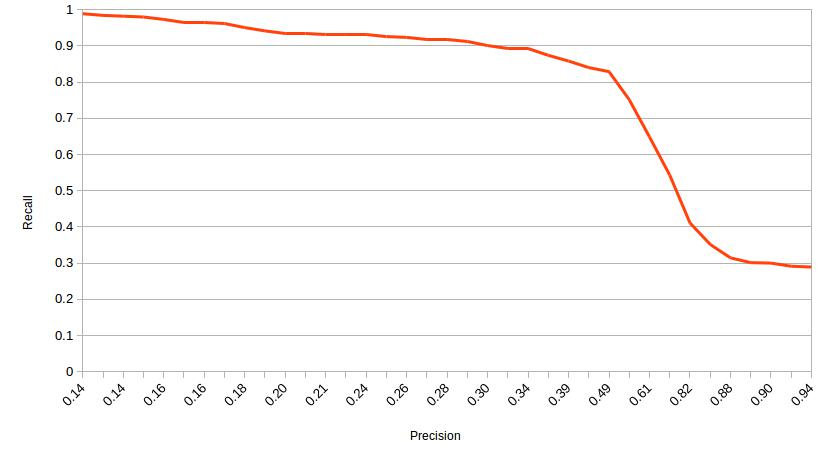
\includegraphics[width=\textwidth]{precRec.jpg}
\makeatletter
\let\@currsize\normalsize
\caption{Precision Recall Curve for Weighted Genre Estimation}
\label{fig:precRec}
\end{figure}

\begin{figure}
\centering
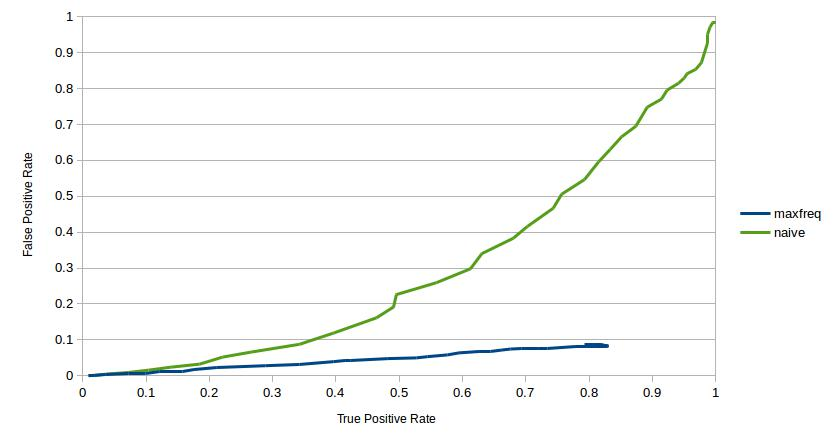
\includegraphics[width=\textwidth]{roc.jpg}
\makeatletter
\let\@currsize\normalsize
\caption{ROC curve for max frequency and naive genre estimation}
\label{fig:roccurve}
\end{figure}

\newpage 

\subsection{Results on exploratory query analysis}

\noindent In order to estimate the efficacy of the Modulo7 SQL querying, certain customized querying experiments are conducted. In order to ascertain the relevance of the statistic extraction \ref{statistic} and criteria estimation \ref{criteria}, certain queries were designed and cross checked with the tags associated with that song (since meta data tags come along with the songs in the million song data set). For example based on a prior statement made about intervals expressing the mood of a song in \ref{intervals} , we can estimate a rock song based on a query : select mp3 from database where power index > k where k is some thresh hold. This particular experiment involves exploring for a reasonable estimate of k to ascertain rock songs from non-rock songs. The ground truth would be the genre labels extracted in \ref{genrelabels} or the last fm dataset tags \cite{msd} depending on the query context. \textbf{Its important to note that this experiment is exploratory and novel in nature and hence there is no pre-existing framework/methodology or approach to compare against.}\\

\noindent The query and their equivalent statement are -++listed and the accuracies for simple queries are listed below:- \\

\begin{table}[h]
\begin{center}
    \begin{tabular}{| l | l | l | l | l |}
    \hline
    Purpose &  Query & precision  & recall & ground truth estimate \\ \hline
    Rock Song ID &  Q1 & 0.13  & 0.98 & Song tags : "rock" / "pop\_rock" \\ \hline
    Sad Song ID &  Q2 & 0.02  & 0.44 & Song tags : "sad" / "sad\_song" \\ \hline
    Happy Song ID &  Q3 & 0.018  & 0.4 & Song tags : "happy" / "happy\_song" \\
    \hline
    \end{tabular}
\end{center}
\caption{Results for the exploratory query analysis}
\end{table}

\noindent We define Q1, Q2 and Q3 as follows

\begin{enumerate}
\item [Q1] select mp3 from default\_database where powerindex $>$ 0.61;
\item [Q2] select mp3 from default\_database where sadnessindex $>$ 0.15 and scale = minor;
\item [Q3] select mp3 from default\_database where happinessindex $>$ 0.11 and scale = major;
\end{enumerate}

From these results we can conclude the following : 

\begin{enumerate}
\item A cursory analysis of the data set revealed that 57\% of all songs in the data set are classified as rock or pop rock. Hence the high optimal value of k for powerindex is justified given the higher concentration of rock songs. 
\item While recall is high (especially for rock songs), precision is low for all queries in this analysis. This would entail that while the relevant songs are indeed retrieved, many irrelevant songs are also retrieved which satisfy the criteria. This could be resolved by compounding the query with criteria/statistics which filter out the false positives. 
\end{enumerate}

\section{Results on melodic alignment and similarities over sub melodies}

\noindent A micro experiment was run to show the extensibility of Modulo7 for the purpose of melodic alignment. Its often important to ascertain which regions of a melody are similar to which other regions of a melody. For this experiment, the Smith Waterman algorithm \ref{SMAlgorithm} is used for similarity computation and representing regions of melodies that are similar to each other. 

\section{Results on KK Tonality Profiles algorithm for Key Estimation}

\noindent In order to test the KK Tonality algorithm given in \ref{kktonality}, Modulo7 is benchmarked against a big subset of the Wikifonia data set of lead sheets in the compact mxl format (variant of the music xml format) \cite{WikifoniaDataset}. The original dataset of the Wikifonia is now no longer available but a sizable subset of 6715 songs are currently down loadable and copyright free. Out of this set, 1314 have key signatures embedded in the song sources. The experiment involves comparing the key signatures embedded inside the key signatures versus the implied key signatures the KK Tonality estimates from the pitch histogram of the songs parsed from this source. A special MXL parser (a minor variant of the music xml parser) was developed for this purpose. The scoring scheme for this experiment was simple, if the key signature was correctly identified then score of 1 otherwise score of 0. In this particular dataset, key signatures are partially known (\textbf{since the number of sharps or flats in the key signatures are always encoded in music xml files} so only relative major/minor are needed to be ascertained). As a consequence only two choices are to be made between key signatures for each file giving a baseline of 50 percent. In this particular example, KK Tonality's performance is how well it can distinguish between relative minors and majors. \\\\
After running the KK Tonality algorithm on the wikifonia dataset, 1129 out the total 1314 key signatures are correctly identified leading to an accuracy of \text{85.9 percent}. This is commensurate with the reported accuracies in \cite{kkTonalityKeyFinding}. The novelty of this experiment stems from the fact that KKTonality profiles algorithm was not successfully run against a large scale database successfully in literature. 

\section{Results on CPU and Memory and Disk space compared against jMIR}

\noindent In order to compare the memory and disk space requirements, Modulo7 was tested against its closest competitor jMIR's \cite{jMIR} jSymbolic component. Both frameworks are written in Java and both involve extraction of features(although that is not an end goal for Modulo7). However jMIR is more exhaustive in what features it extracts so only a subset of those that are also extracted by Modulo7 are considered. Out of the total 111 features that are implemented in jSymbolic \cite{jSymbolic}, 23 features were identified as implemented as internal computation within the Modulo7 indexers and/or querying engine. \textbf{Its important to note that unlike jMIR, Modulo7 is not an exhaustive feature extractor}. The features identified are stated below \\
\begin{enumerate}
\item 1 feature for duration of song
\item 2 features for average melodic intervals, note duration
\item 1 feature for Meter classification (simple or compound)
\item 1 feature for lengths of melodic archs in midi files
\item 1 feature for initial tempo of song
\item 4 features for melodic intervals (thirds, fifths, octaves and intervals in the bass line)
\item 2 features for maximum and minimum durations of notes in the song
\item 3 features for most commonly occurring pitch, pitch class and melodic interval
\item 3 features for ranges, namely primary register, range of highest and lowest voices
\item 1 feature for time signature
\item 4 features for checking for voice equality in the following categories : melodic leaps, note duration, number of notes and range \\
\end{enumerate}
\noindent In order to compare the frameworks, jProfiler was to profile for max CPU utilization, average Java Heap Memory usage and time taken for both frameworks over different sized subsets of the Saarland Music Data (SMD) Dataset \cite{saarlandmsd}. In order to protect against background process interference, the frameworks were ran on AWS EC2 m4x.large instances (dual core 2.4 GHz Intel Xeon® E5-2676 v3 Haswell processors and 8 GB DDR3 RAM). We plot the average memory consumed, CPU load and time taken in seconds as a function of dataset size (over monotonically increasing subset sizes of the SMD dataset). We ignore IO performance since in this experiment, IO is only utilized when pushing output to disk, which is not taken as a metric of evaluation. No data sets involving music xml files were chosen, as jSymbolic does not support music xml files. 

\begin{figure}
\centering
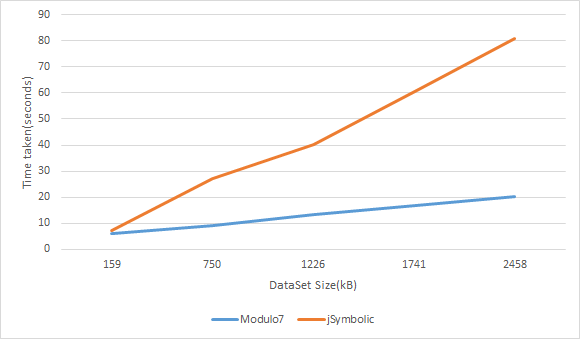
\includegraphics[width=\textwidth]{TimeTaken.png}
\makeatletter
\let\@currsize\normalsize
\caption{Modulo7 vs jSymbolic for time taken to generate features}
\label{fig:time}
\end{figure}

\begin{figure}
\centering
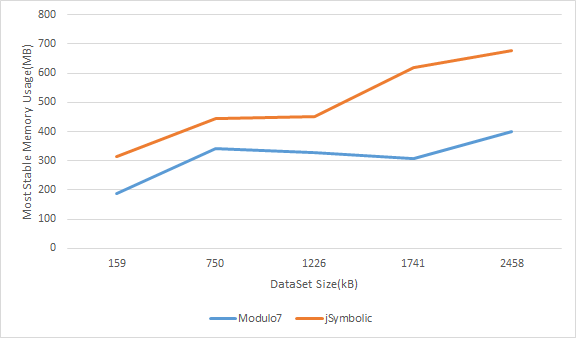
\includegraphics[width=\textwidth]{MemoryTaken.png}
\makeatletter
\let\@currsize\normalsize
\caption{Modulo7 vs jSymbolic for average memory utilized}
\label{fig:mem}
\end{figure}

\begin{figure}
\centering
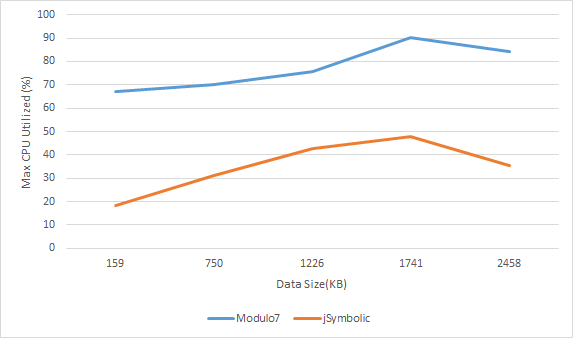
\includegraphics[width=\textwidth]{CPUUsage.png}
\makeatletter
\let\@currsize\normalsize
\caption{Modulo7 vs jSymbolic for maximum CPU utilized utilized}
\label{fig:cpu}
\end{figure}

\newpage

\noindent From these graphs we can conclude the following :-

\begin{enumerate}
\item Modulo7 is much faster than jSymbolic when computing core features and both of them scale linearly. The rate of increase for Modulo7 is lower, and hence Modulo7 scales better for larger datasets as compared to jSymbolic.
\item jSymbolic under utilizes CPU for computing features whereas Modulo7 is optimal in terms of CPU usage. The profiling results revealed that jSybmolic is single threaded and contains no caching mechanism for storing features (leading to re-computation of features that are dependencies of other features)
\item jSymbolic consumes more Java Heap memory during execution on average.
\end{enumerate}


 


